\textbf{Ejemplo 1}\\
Si invierto hoy un capital de 1.000.000 COP, cuánto capital podré retirar en 18 meses suponiendo que el capital invertido gana el 24\% (nasv) nominal anual semeste vencido? \\ \\
%\newpage %USAR SOLO SI EL SOLUCIÓN QUEDA SOLO Y ES NECESARIO BAJARLO A LA SIGUIENTE PAGINA
\textbf{Solución.}\\
%La tabla ira centrada
\begin{center}
 \renewcommand{\arraystretch}{1.5}% Margenes de las celdas
 %Creación de la cuadricula de 3 columnas
 \begin{longtable}[H]{|p{0.5\linewidth}|p{0.5\linewidth}|}
  \hline
  \multicolumn{2}{|c|}{\cellcolor[HTML]{FFB183}\textbf{1. Declaración de variables}}                  \\ \hline
  $n = 3 \hspace{1mm} psv$                                      & $VF =  1{.}000{.}000$ COP             \\
  $j = 24\% \hspace{1mm} nasv \equiv i = 12\% \hspace{1mm} psv$ & $VP =  ?$ COP                       \\ \hline
  \multicolumn{2}{|c|}{\cellcolor[HTML]{FFB183}\textbf{2. Tabla de flujo de caja}}                    \\ \hline
  \multicolumn{2}{|p{\columnwidth}|}{
  \begin{center}
   \begin{tabular}{|c|c|}
    \hline
    Periodo (psv) & Flujo          \\ \hline
    $0$           &  1.000.000 COP             \\ \hline
    $1$           &  COP -            \\ \hline
    $2$           &  COP -            \\ \hline
    $3$           &  ? COP \\ \hline
   \end{tabular}
  \end{center}
  }                                                                                                   \\ \hline
  \multicolumn{2}{|c|}{\cellcolor[HTML]{FFB183}\textbf{3. Fórmulas utilizadas}}                       \\ \hline
  \multicolumn{2}{|l|}{Mediante el uso de Excel:}                                                     \\
  \multicolumn{2}{|l|}{VF (Valor futuro): Devuelve el valor futuro para una inversión}              \\ \hline
  \multicolumn{2}{|c|}{\cellcolor[HTML]{FFB183}\textbf{4. Desarrollo en Excel}}                       \\ \hline
  \multicolumn{2}{|l|}{Se aplicará la función VF de la siguiente forma:}                              \\
  \multicolumn{2}{|c|}{ 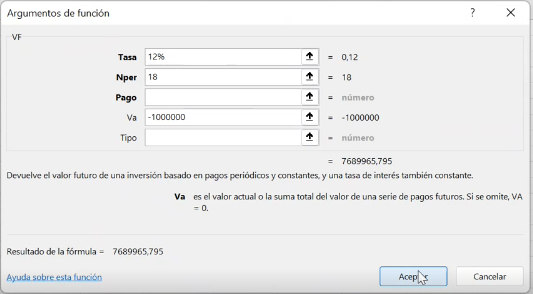
\includegraphics[trim=-5 -5 -5 -5 ,width=1\columnwidth]{1/Ejem1.PNG}}         \\
  \multicolumn{2}{|l|}{=VA (0,12; 18; -1000000) con referencia en la hoja de Excel usada para el ejercicio.} \\ \hline
  \multicolumn{2}{|c|}{\cellcolor[HTML]{FFB183}\textbf{5. Respuesta}}                                 \\ \hline
  \multicolumn{2}{|c|}{El valor futuro (VF) es de  7.689.965 COP.}               \\ \hline
  \multicolumn{2}{|c|}{\cellcolor[HTML]{FFB183}\textbf{6. Gráfica}}                                   \\ \hline
  \multicolumn{2}{|c|}{No es necesaria la realización de una gráfica para este ejercicio.}            \\ \hline
 \end{longtable}
 %\newline \newline %USARLO SI CREES QUE ES NECESARIO
\end{center}
